\newcommand{\tikzabstractconfig}[5]{% x, y, val1, val2, q, x1, y1
	\begin{tikzpicture}
		\draw (#1,#2) rectangle (1 + #1,0.5 +#2);
		\draw (#1,-0.5 + #2) rectangle (1 +#1 ,#2);
		\node[] (x1) at (0.5 + #1, 0.15 +#2) {#3};
		\node[] (x2) at (0.5 +#1 , 0.15- 0.5 +#2) {#4};
		\node [] (q) at (0.5 +#1, 0.7+#2) {#5};
	\end{tikzpicture}
}

\newcommand{\tikzvalue}[4]{% x, y, length, val
	\begin{tikzpicture}
		\node [] (v) at (#1 + #3 + 0.3, #2 + 1.2) {$\mathbf{v}= #4$};
	\end{tikzpicture}
}

\newcommand{\tikzspec}[4]{% x, y, length, spec
	\begin{tikzpicture}
		\node [] (sp) at (#3 /2, #2 - 0.2) {#4};
	\end{tikzpicture}
}

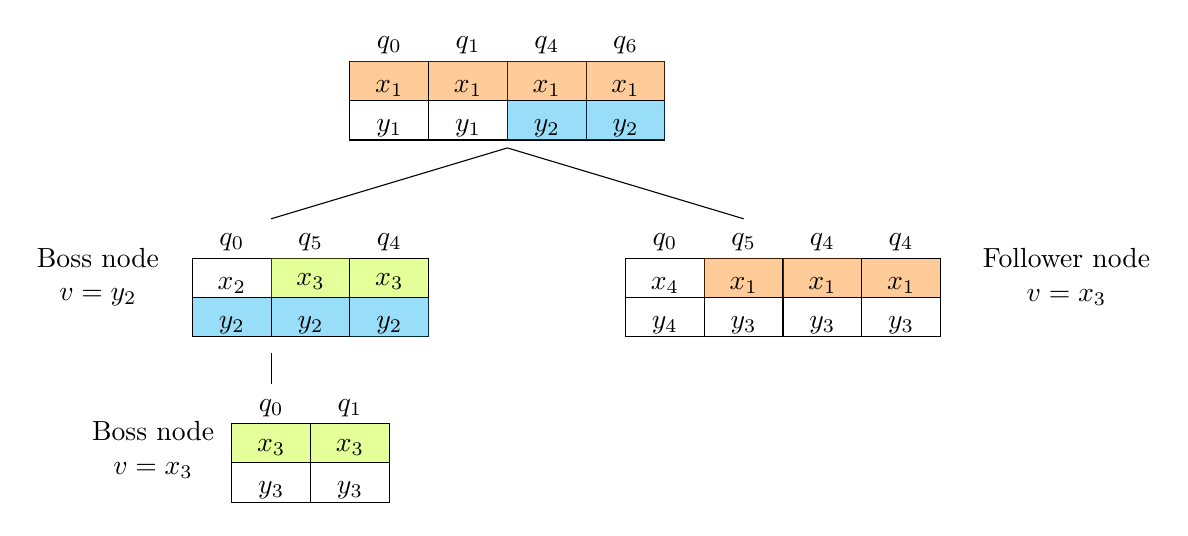
\begin{tikzpicture}
	
	

%	
%	\tikzabstractconfig{0}{0}{$x_1$}{$y_1$}{$q_0$}
%	\tikzabstractconfig{1}{0}{$x_1$}{$y_1$}{$q_1$}
%	\tikzabstractconfig{2}{0}{$x_1$}{$y_2$}{$q_4$}
%	\tikzabstractconfig{3}{0}{$x_1$}{$y_2$}{$q_6$}


	\draw (0,0) rectangle (1,0.5);
	\draw[fill = orange, opacity=0.4]  (0,0) rectangle (1,0.5);
	\draw (0,-0.5 ) rectangle (1 ,0);
	\node[] (x1) at (0.5, 0.15) {$x_1$};
	\node[] (x2) at (0.5 , 0.15- 0.5) {$y_1$};
	\node [] (q) at (0.5 , 0.7) {$q_0$};
	
	\draw (1,0) rectangle (2,0.5);
	\draw[fill = orange, opacity=0.4]  (1,0) rectangle (2,0.5);
	\draw (1,-0.5 ) rectangle (2 ,0);
	\node[] (x1) at (1.5, 0.15) {$x_1$};
	\node[] (x2) at (1.5 , 0.15- 0.5) {$y_1$};
	\node [] (q) at (1.5 , 0.7) {$q_1$};
	
	\draw (2,0) rectangle (3,0.5);
	\draw[fill = orange, opacity=0.4] (2,0) rectangle (3,0.5);
	\draw (2,-0.5 ) rectangle (3 ,0);
	\draw[fill = cyan, opacity=0.4] (2,-0.5 ) rectangle (3 ,0);
	\node[] (x1) at (2.5, 0.15) {$x_1$};
	\node[] (x2) at (2.5 , 0.15- 0.5) {$y_2$};
	\node [] (q) at (2.5 , 0.7) {$q_4$};
	
	
	\draw[] (3,0) rectangle (4,0.5);
	\draw[fill = orange, opacity=0.4] (3,0) rectangle (4,0.5);
	\draw (3,-0.5 ) rectangle (4 ,0);
	\draw[fill = cyan, opacity=0.4]  (3,-0.5 ) rectangle (4 ,0);
	\node[] (x1) at (3.5, 0.15) {$x_1$};
	\node[] (x2) at (3.5 , 0.15- 0.5) {$y_2$};
	\node [] (q) at (3.5 , 0.7) {$q_6$};
	
    \draw (2, -0.6) -- (-1, -1.5);
    \draw (2, -0.6) -- (5, -1.5);
    
    
    
    \node [] (sp) at (-3.2, -2) {Boss node};
    \node [] (sp) at (-3.2, -2.5) {$v = y_2$};
    
    \draw (-2,-2.5) rectangle (-1,-2);
    \draw  [fill = cyan, opacity=0.4] (-2,-3 ) rectangle (-1 ,-2.5);    
    \draw  (-2,-3 ) rectangle (-1 ,-2.5);
    \node[] (x1) at (-1.5, 0.15 - 2.5) {$x_2$};
    \node[] (x2) at (-1.5 , 0.15- 0.5 - 2.5) {$y_2$};
    \node [] (q) at (-1.5 , 0.7 - 2.5) {$q_0$};
    
    \draw (-1,-2.5) rectangle (0,-2);
     \draw [fill = lime, opacity=0.4] (-1,-2.5) rectangle (0,-2);
    \draw [fill = cyan, opacity=0.4] (-1,-3 ) rectangle (0 ,-2.5);    
    \draw (-1,-3 ) rectangle (0 ,-2.5);
    \node[] (x1) at (-0.5, 0.2 -2.5) {$x_3$};
    \node[] (x2) at (-0.5 , 0.15- 0.5 - 2.5) {$y_2$};
    \node [] (q) at (-0.5 , 0.7-2.5) {$q_5$};
    
    \draw [fill = lime, opacity=0.4] (0,-2.5) rectangle (1,-2);
    \draw (0,-2.5) rectangle (1,-2);
    \draw (0,-3 ) rectangle (1 ,-2.5);
    \draw[fill = cyan, opacity=0.4] (0,-3 ) rectangle (1 ,-2.5);
    \node[] (x1) at (0.5, 0.2 -2.5) {$x_3$};
    \node[] (x2) at (0.5 , 0.15- 0.5 - 2.5) {$y_2$};
    \node [] (q) at (0.5 , 0.7-2.5) {$q_4$};
    
    
    \draw (-1, -3.2) -- (-1, -3.6);
    
   
   \node [] (sp) at (-2.5, -4.2) {Boss node};
   \node [] (sp) at (-2.5, -4.7) {$v = x_3$};
   
   
   \draw (-1.5,-4.6) rectangle (-0.5,-4.1);
   \draw [fill = lime, opacity=0.4] (-1.5,-4.6) rectangle (-0.5,-4.1);
   \draw (-1.5,-5.1 ) rectangle (-0.5 ,-4.6);
   \node[] (x1) at (-1, 0.2 -4.6) {$x_3$};
   \node[] (x2) at (-1 , 0.15- 0.5 - 4.6) {$y_3$};
   \node [] (q) at (-1 , 0.7-4.6) {$q_0$};
    
    
    \draw (-0.5,-4.6) rectangle (0.5,-4.1);
    \draw [fill = lime, opacity=0.4] (-0.5,-4.6) rectangle (0.5,-4.1);
    \draw (-0.5,-5.1 ) rectangle (0.5 ,-4.6);
    \node[] (x1) at (0, 0.2 -4.6) {$x_3$};
    \node[] (x2) at (0 , 0.15- 0.5 - 4.6) {$y_3$};
    \node [] (q) at (0 , 0.7-4.6) {$q_1$};
	
%	\draw (-3,-2) rectangle (-2,0.5 -2);
%	\draw (-3,-0.5 -2) rectangle (1 -3 ,-2);
	%\node[] (x1) at (0.5 + #1, 0.15 +#2) {#3};
	%\node[] (x2) at (0.5 +#1 , 0.15- 0.5 +#2
%	
%	\tikzabstractconfig{-3}{-2}{$x_1$}{$y_1$}{$q_0$} 
%	\tikzabstractconfig{-2}{-2}{$x_1$}{$y_1$}{$q_1$}
	
	
	\draw (3.5,-2.5) rectangle (4.5,-2);
	\draw (3.5,-3 ) rectangle (4.5 ,-2.5);
	\node[] (x1) at (4, 0.15 - 2.5) {$x_4$};
	\node[] (x2) at (4 , 0.15- 0.5 - 2.5) {$y_4$};
	\node [] (q) at (4 , 0.7 - 2.5) {$q_0$};
	
	\draw (4.5,-2.5) rectangle (5.5,-2);
	\draw[fill = orange, opacity=0.4]  (4.5,-2.5) rectangle (5.5,-2);
	\draw (4.5,-3 ) rectangle (5.5 ,-2.5);
	\node[] (x1) at (5, 0.15 - 2.5) {$x_1$};
	\node[] (x2) at (5 , 0.15- 0.5 - 2.5) {$y_3$};
	\node [] (q) at (5 , 0.7 - 2.5) {$q_5$};

	\draw (5.5,-2.5) rectangle (6.5,-2);
	\draw[fill = orange, opacity=0.4] (5.5,-2.5) rectangle (6.5,-2);
	\draw (5.5,-3 ) rectangle (6.5 ,-2.5);
	\node[] (x1) at (6, 0.15 - 2.5) {$x_1$};
	\node[] (x2) at (6 , 0.15- 0.5 - 2.5) {$y_3$};
	\node [] (q) at (6 , 0.7 - 2.5) {$q_4$};
	
	\draw[fill = orange, opacity=0.4] (6.5,-2.5) rectangle (7.5,-2);
	\draw (6.5,-2.5) rectangle (7.5,-2);
	\draw (6.5,-3 ) rectangle (7.5 ,-2.5);
	\node[] (x1) at (7, 0.15 -2.5) {$x_1$};
	\node[] (x2) at (7 , 0.15- 0.5 - 2.5) {$y_3$};
	\node [] (q) at (7 , 0.7-2.5) {$q_4$};
	
	\node [] (sp) at (9.1, -2) {Follower node};
	\node [] (sp) at (9.1, -2.5) {$v = x_3$};
	
%	\draw (7.5,-2.5) rectangle (8.5,-2);
%	\draw (7.5,-3 ) rectangle (8.5,-2.5);
%	\node[] (x1) at (8, 0.2 -2.5) {$x'_2$};
%	\node[] (x2) at (8 , 0.15- 0.5 - 2.5) {$y_2$};
%	\node [] (q) at (8 , 0.7-2.5) {$q_4$};
%	

	
\end{tikzpicture}